%% LaTeX2e class for student theses
%% sections/main/5_design.tex
%%
%% Karlsruhe University of Applied Sciences
%% Faculty of Computer Science and Business Information Systems
%%
%% --------------------------------------------------------
%% | Derived from sdqthesis by Erik Burger burger@kit.edu |
%% --------------------------------------------------------

\chapter{Design}
\label{ch:Design}

This chapter presents a design that takes into account the processes cross-checked with existing approaches for reservation systems in the context of \acrshort{emobility}, as discussed in chapter \ref{ch:Literature Review}. 
Building upon the definitions of requirements and use cases outlined in Chapter \ref{ch: Requirements Engineering}, the following Sections deal with the conceptualization of the required entities, such as the reservation, as well as the functionality for sufficient management capabilities of the underlying charging infrastructure.
Furthermore, the mockups created during the theoretical part of this work are associated with the corresponding capabilities that the system has to satisfy. These interfaces, representing the flow of user interaction, are combined with the related processes implemented in the underlying system.

\section{Reservation}
\label{ch:Design:sec:Reservation}

As a fundamental unit, the reservation entity and its constituents serve as the foundation for the design process.  
Hence, multiple sources, such as the \acrshort{ocpp} standard, which is employed by most \acrshortpl{cs}, and the associated research in chapter \ref{ch:Literature Review}, are given primary consideration.
To cover the basic functionality for interacting with the underlying charging infrastructure, the reservation must contain specific properties that enable an unambiguous mapping between the entities provided in the standard solutions and those internal to the system.
Considering the absence of features not covered by existing standards, this thesis introduces several properties as a dedicated extension to the existing work, which should provide further possibilities in the management of reservations and related infrastructure.
Starting with the requirements for compliance with version 1.6 of the \acrshort{ocpp} standard, the selection inside Table \ref{tab:reservation-ocpp-properties} includes the same essential information as the aforementioned protocol.

\begingroup
\setlength{\tabcolsep}{10pt} % Default value: 6pt
\renewcommand{\arraystretch}{1.5} % Default value: 1
\begin{table}[h]
    \centering
    \caption{Reservation properties based on \textit{Reserve Now} operation in \cite{noauthor_ocpp_nodate}.}
    \begin{tabular}{c|m{10cm}}
        Property & Description \\ \hline
        \acrshort{id} & Distinct identifier for the reservation within the \acrshort{cs} and the system \\
        Charging Station \acrshort{id} & Association to the corresponding \acrshort{cs} \\
        Connector \acrshort{id} & Association with the relevant reserved connector \\
        Tag \acrshort{id} & Association with the \acrshort{rfid} tag for the user \\
        Parent Tag \acrshort{id} & Association with the superior \acrshort{rfid} tag \\
        Expiry Date & Date when the reservation expires
    \end{tabular}
    \label{tab:reservation-ocpp-properties}
\end{table}
\endgroup

\newpage

\noindent Based on these standard properties required for an \acrshort{ocpp} reservation, the author proposes the extensions listed in Table \ref{tab:reservation-extended-properties}.

\begingroup
\setlength{\tabcolsep}{10pt} % Default value: 6pt
\renewcommand{\arraystretch}{1.5} % Default value: 1
\begin{table}[h]
    \centering
    \caption{Reservation properties extending \acrshort{ocpp} protocol in version 1.6.}
    \begin{tabular}{c|m{10cm}}
        Property & Description \\ \hline
        From Date & Date the reservation begins \\ 
        To Date & Date the reservation ends \\
        Arrival Time & Dedicated time the reservation starts \\
        Departure Time & Dedicated time the reservation ends \\
        Status & Reservation status according to \ref{ch:Design:sec:Reservation:ssec:Reservation Status} \\
        Type & Type of reservation according to \ref{ch:Design:sec:Reservation:ssec:Reservation Types} \\
        Car \acrshort{id} & Association to users car 
    \end{tabular}
    \label{tab:reservation-extended-properties}
\end{table}
\endgroup

\noindent Especially these enhancements should enable the system user to make an advance reservation, in addition to the already supported immediate reservations for locking connectors directly, by booking a single or a recurring reservation(s) within a selected date range and time slot.
Furthermore, the option to add the car to the booking should enable the compatibility of the reservation system for the integration of \acrshort{sg} applications, e.g. providing \acrshort{v2g} operations.
The introduction of the \textit{status} and \textit{type} properties serves as markers to distinguish between reservation types and the current status of the reservation. The details of this are discussed below.
Properties such as prioritizing reservations for different categories of users or integrating a pricing scheme are not covered by this work and could be developed as part of future work to extend this reservation system approach.
To fully understand the new relationships between entities in the system and their use in the reservation framework, the next subsection outlines these new associations.

\subsection{Entity Relationships}
\label{ch:Design:sec:Reservation:ssec:Entity Relationships}

For the purpose of arranging the properties and entities within the reservation module and the rest of the system, it is necessary to examine the relationships that the specific entities, such as the \acrshort{cs} or a \acrshort{rfid} tag, have with a reservation and the quantity in which they can be used.
For presenting this type of mapping concerning the relationships, they are depicted as an entity relationship diagram to show the respective connections and to illustrate them in the Figure \ref{fig:entity-relationship-diagram}.
Stated as a constraint by the \acrshort{ocpp} standard, it is intended that the reservation can only reserve a particular \acrshort{cs} and connector during a given time. Additionally, either an individual user, identified by their associated \acrshort{rfid} tag or a group of users linked to a parental \acrshort{rfid} tag that represents this subset, may use the reservation. The chosen vehicle must also adhere to these restrictions.

\begin{figure}[h]
    \centering
    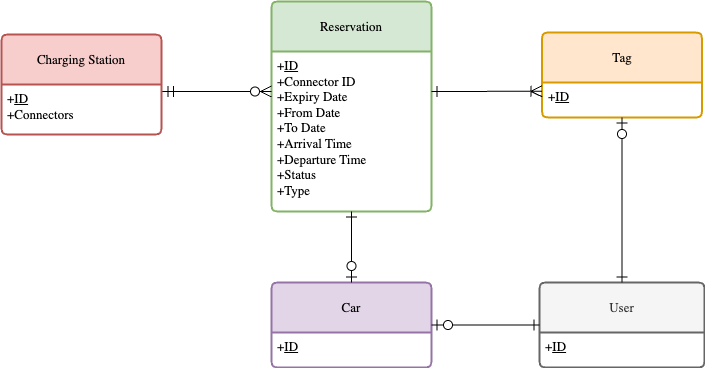
\includegraphics[scale=0.4]{resources/images/main/5_design/Entities.png}
    \caption{Entities and their relationships with the corresponding quantities.}
    \label{fig:entity-relationship-diagram}
\end{figure}

\noindent Beyond the relationships established during this design process, the succeeding subsections detail the newly introduced properties in terms of their relevance to later implementations and the functionality they provide.

\subsection{Reservation Status}
\label{ch:Design:sec:Reservation:ssec:Reservation Status}

According to the findings of Flocea et al. \cite{flocea_electric_2022}, the reservation process goes through several stages before it is completed. These stages can be depicted as a status, which indicates where the reservation is currently located in the reservation process and provides an overview of the options available to the relevant user or the system itself to interact with the reservation.
Thus, the study mentioned above introduced four distinct states, distinguishing between \textit{New}, \textit{Done}, \textit{In progress}, and \textit{Cancelled}.
Considering these pre-existing states, this thesis proposes an extension that allows a more granular treatment of a reservation during its life cycle. Besides breaking down the particular steps within the life of a reservation, these additional states allow further functionality in terms of mitigating undesired behavior and enforcing software-based rules in terms of the design parameter \textit{Enforceability} mentioned later.

\begingroup
\setlength{\tabcolsep}{10pt} % Default value: 6pt
\renewcommand{\arraystretch}{1.5} % Default value: 1
\begin{table}[h]
    \centering
    \caption{Introduced reservation states to extend the reservation life cycle.}
    \begin{tabular}{c|c|m{7cm}}
        Reservation Status & Equivalent in \cite{flocea_electric_2022} & Description \\ \hline
        Done & - & \acrshort{evu} was present and charged the \acrshort{ev} \\
        Scheduled & New & Planned reservations whose start date has not yet been reached \\
        In Progress & In progress & Reservation currently in progress \\
        Cancelled & Cancelled & The reservation has been cancelled \\
        Expired & - & The reservation has reached its expiration date. \\
        Unmet & - & The \acrshort{evu} did not arrive punctually
    \end{tabular}
    \label{tab:reservation-states}
\end{table}
\endgroup

\noindent Taking into account the current states, the proposed extensions additionally cover the scenarios of a user not arriving on time, the reservation itself expiring, the reservation being successfully fulfilled, and partially the scheduled state until the start of the reserved time slot. 
These aspects are not considered by Forcea et al. and should be integrated to address certain situations.
To characterize these particular situations, the state diagram below, shown in Figure \ref{fig:reservation-states}, provides an overview of the possible transitions according to the conditions that must be met.

\begin{figure}[h]
    \centering
    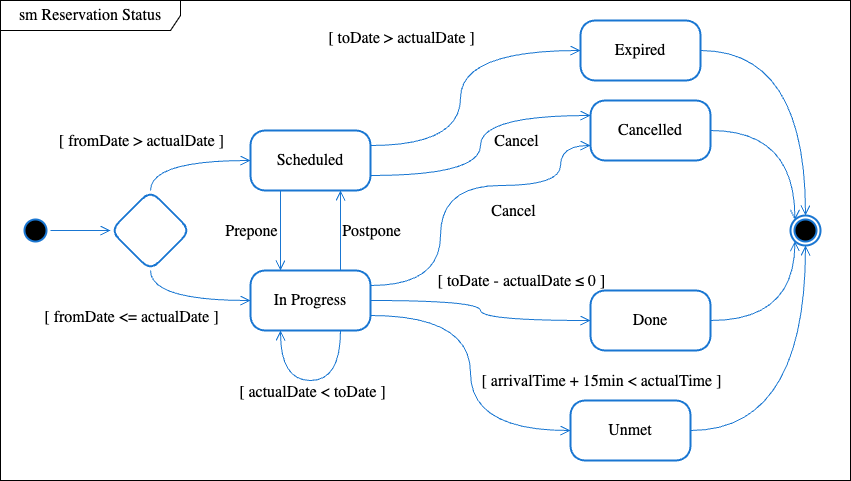
\includegraphics[scale=0.4]{resources/images/main/5_design/ReservationStatusStates.png}
    \caption{State diagram with the corresponding state transitions for the possible reservation states within the implementation.}
    \label{fig:reservation-states}
\end{figure}

\noindent Not every reservation undergoes the same stages as depicted above due to its specific type. To provide an overview of each reservation type included in the reservation system design, the next subsection offers guidance on the potential variations.

\newpage

\subsection{Reservation Types}
\label{ch:Design:sec:Reservation:ssec:Reservation Types}

As outlined by Basmadjian and colleagues, a reservation system can accommodate various types of bookings. In addition to the immediate blocking of resources through the \textit{Ad-Hoc} reservation mechanism, the \textit{Planned} reservation allows for advance booking, opening up a wider range of possibilities for incorporating this functionality into the management of charging infrastructure \cite{basmadjian_interoperable_2019,basmadjian_reference_2020}.
For this purpose, the authors distinguish between reservation types based on their \textit{enforceability} and propose uncertain and guaranteed reservations, which can be combined to form four possible variations.
The \textit{uncertain} reservations cannot guarantee that the reserved \acrshort{cs} and its corresponding parking spot will not be occupied by another vehicle upon arrival, whereas the \textit{guaranteed} reservation ensures this possibility.
Enabling this reliability requires the implementation of additional functionalities, such as the ability to control the physical infrastructure itself.
In this design process, considering no direct access to physical infrastructure services as blockers for parking and similar technologies, the resulting system tries to provide a hybrid reservation type combining the best from the world of \textit{uncertain} and \textit{guaranteed} reservations using only software-based solutions to provide the desired level of \textit{enforceability}.
Building a connection to the types found in the existing literature, the Table \ref{tab:reservation-types} then maps the types used in this design and the subsequent implementation to the existing ones.

\begingroup
\setlength{\tabcolsep}{10pt} % Default value: 6pt
\renewcommand{\arraystretch}{1.5} % Default value: 1
\begin{table}[h]
    \centering
    \caption{Pre-defined reservation types and their mapping to the types used in this work.}
    \begin{tabular}{c|c|m{6.5cm}}
        Reservation Type & Equivalent in \cite{basmadjian_interoperable_2019,basmadjian_reference_2020} & Description \\ \hline
        Reserve Now & Ad-Hoc &Reserving the \acrshort{cs} and its corresponding connector immediately until a specified expiration date is reached. During this time, no other user can use the same connector for charging purposes. \\
        Planned Reservation & Planned & Reserves the \acrshort{cs} and the corresponding connector in advance, enabling recurring reservations by selecting a date range. The connector and the \acrshort{cs} will stay available until the reservation starts.
    \end{tabular}
    \label{tab:reservation-types}
\end{table}
\endgroup

\noindent After introducing the reservation entity, the next section discusses the design of the reservation system, including the relevant processes and system architecture. 

\newpage

\section{Reservation System}
\label{ch:Design:sec:Reservation System}

To empower the user to create and manage their reservations, a reservation system is required. This Section presents a design proposal for the development of the system, which is used as groundwork for the adjacent chapter which aims to put such a system into practice. Firstly, the necessary capabilities considered relevant in this work are discussed, as well as the needed design criteria in terms of the system and its architecture.

\subsection{Design Criteria}
\label{ch:Design:sec:Reservation System:ssec:Design Criteria}

Establishing a functional reservation system for managing charging infrastructure entails the consideration of several design parameters, as outlined by Basmadjian et al.\cite{basmadjian_reference_2020}. Apart from \textit{Enforceability}, \textit{Planning}, \textit{Fees}, aspects such as \textit{Data Availability}, \textit{Roaming} and \textit{Scheduling} are important design parameters that a system design has to address.
Concerning the given options and possibilities present in this design approach, the author of this work opts for the inclusion of \textit{Enforceability} alongside \textit{Planning}, \textit{Data Availability} and \textit{Scheduling}. 
Furthermore, the \acrshort{fcfs} approach has been selected as the most appropriate method for mapping real-world charging session bookings.\\
\noindent In accordance with the terminology employed by \cite{basmadjian_reference_2020}, the system can be defined as follows:

\begin{eqnarray*}
\scriptstyle \biggl\{ "Limited"_{Enforceability}, "Yes"_{Planning}, "No"_{Fee}, "Yes"_{Data\ Availability}, "No"_{Roaming}, "FCFS"_{Scheduling} \biggr\}
\end{eqnarray*}

\noindent To accomplish these goals, the relevant capabilities that attempt to meet these design criteria are outlined below.

\subsection{Management Capabilities}
\label{ch:Design:sec:Reservation System:ssec:Management Capabilities}

When managing various entities, the most commonly utilized functionalities involve creating, updating, or deleting related information. Alongside these processes, the acronym CRUD (create, read, update, delete) is often referenced. In reservation systems, the context permits an additional operation known as cancellation, which invalidates the selected reservation.
As outlined in chapter \ref{ch:Requirements Engineering}, the relevant use cases for the previously mentioned functions are already identified. In addition to these general features, the subsection also explains the use case for enabling them on demand.
Considering these capabilities, the following management capabilities cover at least parts of the design choices such as \textit{Enforceability}, \textit{Planning}, \textit{Data Availability} and \textit{Scheduling}, alongside the scheduling capabilities described in subsection \ref{ch:Design:sec:Reservation System:ssec:Scheduling Capabilities}.

\subsubsection{Create Reservation}
\label{ch:Design:sec:Reservation System:ssec:Management Capabilities:sssec:Create Reservation}

In order to enable all of the subsequent procedures, reservation creation is a mandatory function, which can be considered the initial process. The user inputs their information through the chosen application, followed by system-side validation that leads to further processing in subsequent steps or immediate termination of the process.
Afterward, the system checks for any existing reservations with the same identifier to avoid duplicates and ensure consistency with respect to the underlying database schema. If a reservation with the same identifier exists, the process tests for the same user according to their \acrshort{rfid} tag and updates the reservation according to matching tags or rejects it to prevent privilege escalation.
Next, the system checks for other reservations in the defined time range and ensures that there are no collisions, also known as overlaps, between individual reservations according to their dates and time slots.
Any collisions detected, as well as the escalation of privileges during the update process of an existing reservation, result in a predetermined end.
If no conflict is detected, the reservation type is checked and, in the case of a \textit{ReserveNow} reservation, the encapsulated \textit{ReserveNow} operation defined in the \acrshort{ocpp} standard \cite{noauthor_ocpp_nodate} is triggered. This operation prompts the system to send a request to the relevant \acrshort{cs} to immediately lock the connector. 
Otherwise, when dealing with a \textit{Planned Reservation}, the selected time range will be checked, and if the start time is approaching, similar to the case of a \textit{ReserveNow} reservation, the appropriate \acrshort{cs} is contacted.
Finally, the reservation is saved and a notification, described in more detail in subsection \ref{ch:Design:sec:Reservation System:ssec:Notification Capabilities}, is sent to the user to inform him or her of the successful creation.

\begin{figure}[h]
    \centering
    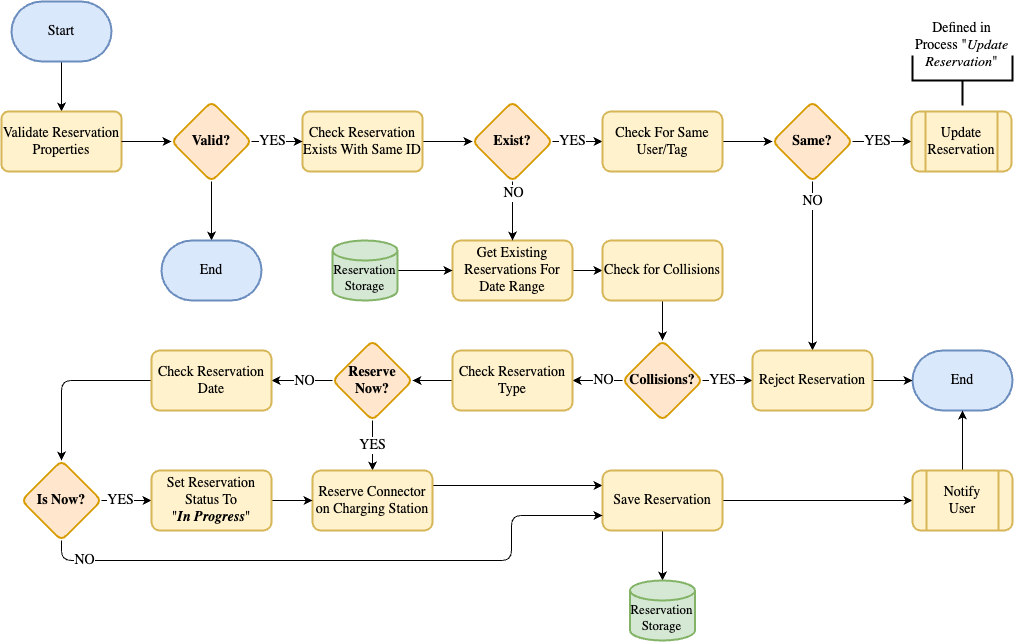
\includegraphics[scale=0.4]{resources/images/main/5_design/processes/ReservationCreate.png}
    \caption{Process flow with all necessary steps to create a reservation.}
    \label{fig:create-reservation-flowchart}
\end{figure}

\noindent To handle the essential inputs, the subsequent mockups offer a suitable user interface encompassing all the required information provided by the user. To address the collection of this vital data, a proposition for the \acrshort{gui} of both the web and mobile app is presented.

\begin{figure}[h]
    \centering
    \begin{subfigure}[c]{0.6\textwidth}
        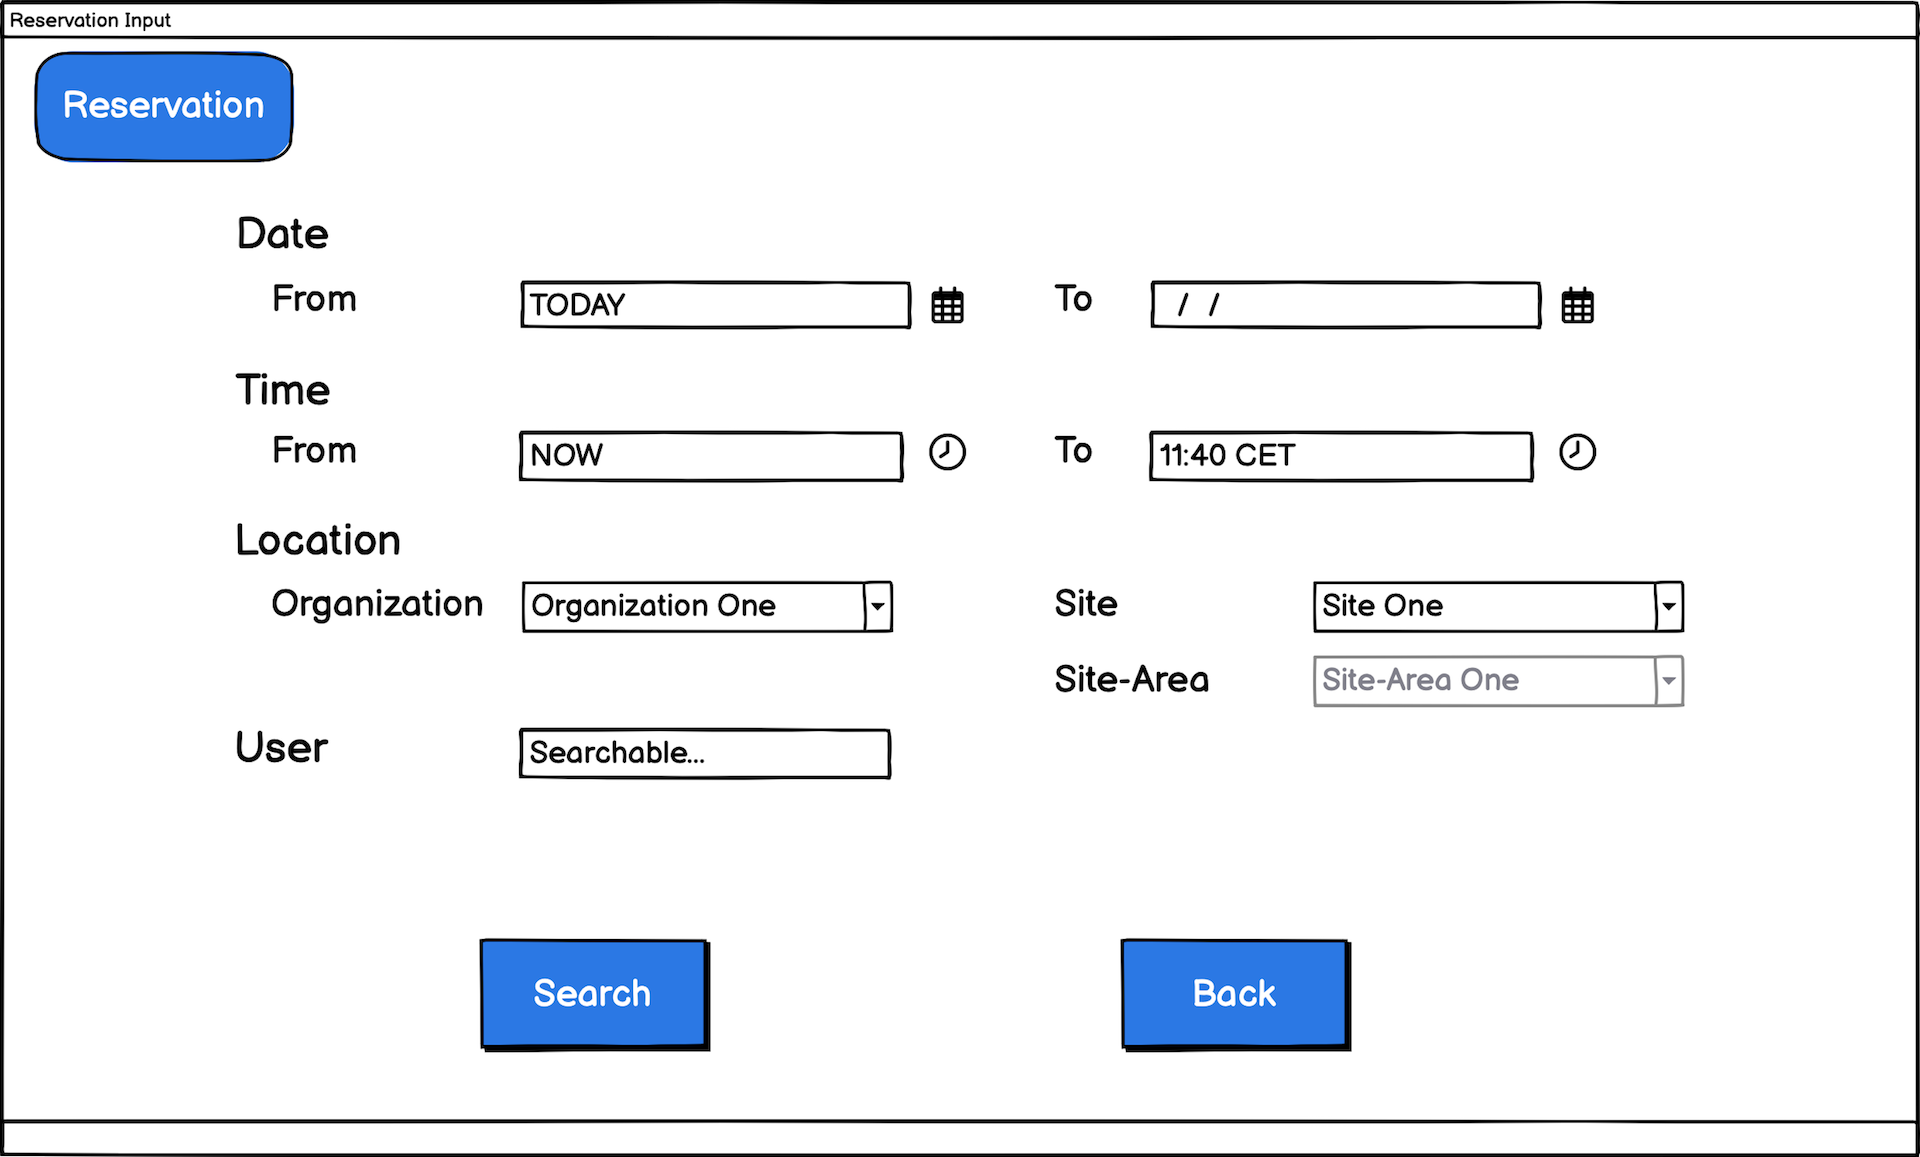
\includegraphics[width=\textwidth]{resources/images/main/5_design/mockups/create_reservation/web/Reservation_Create.png}
        \captionsetup{skip=43pt}
        \caption{Create a reservation in the web application.}
        \label{fig:web-create-reservation-mockup}
    \end{subfigure}
    \hfill
    \begin{subfigure}[c]{0.3\textwidth}
        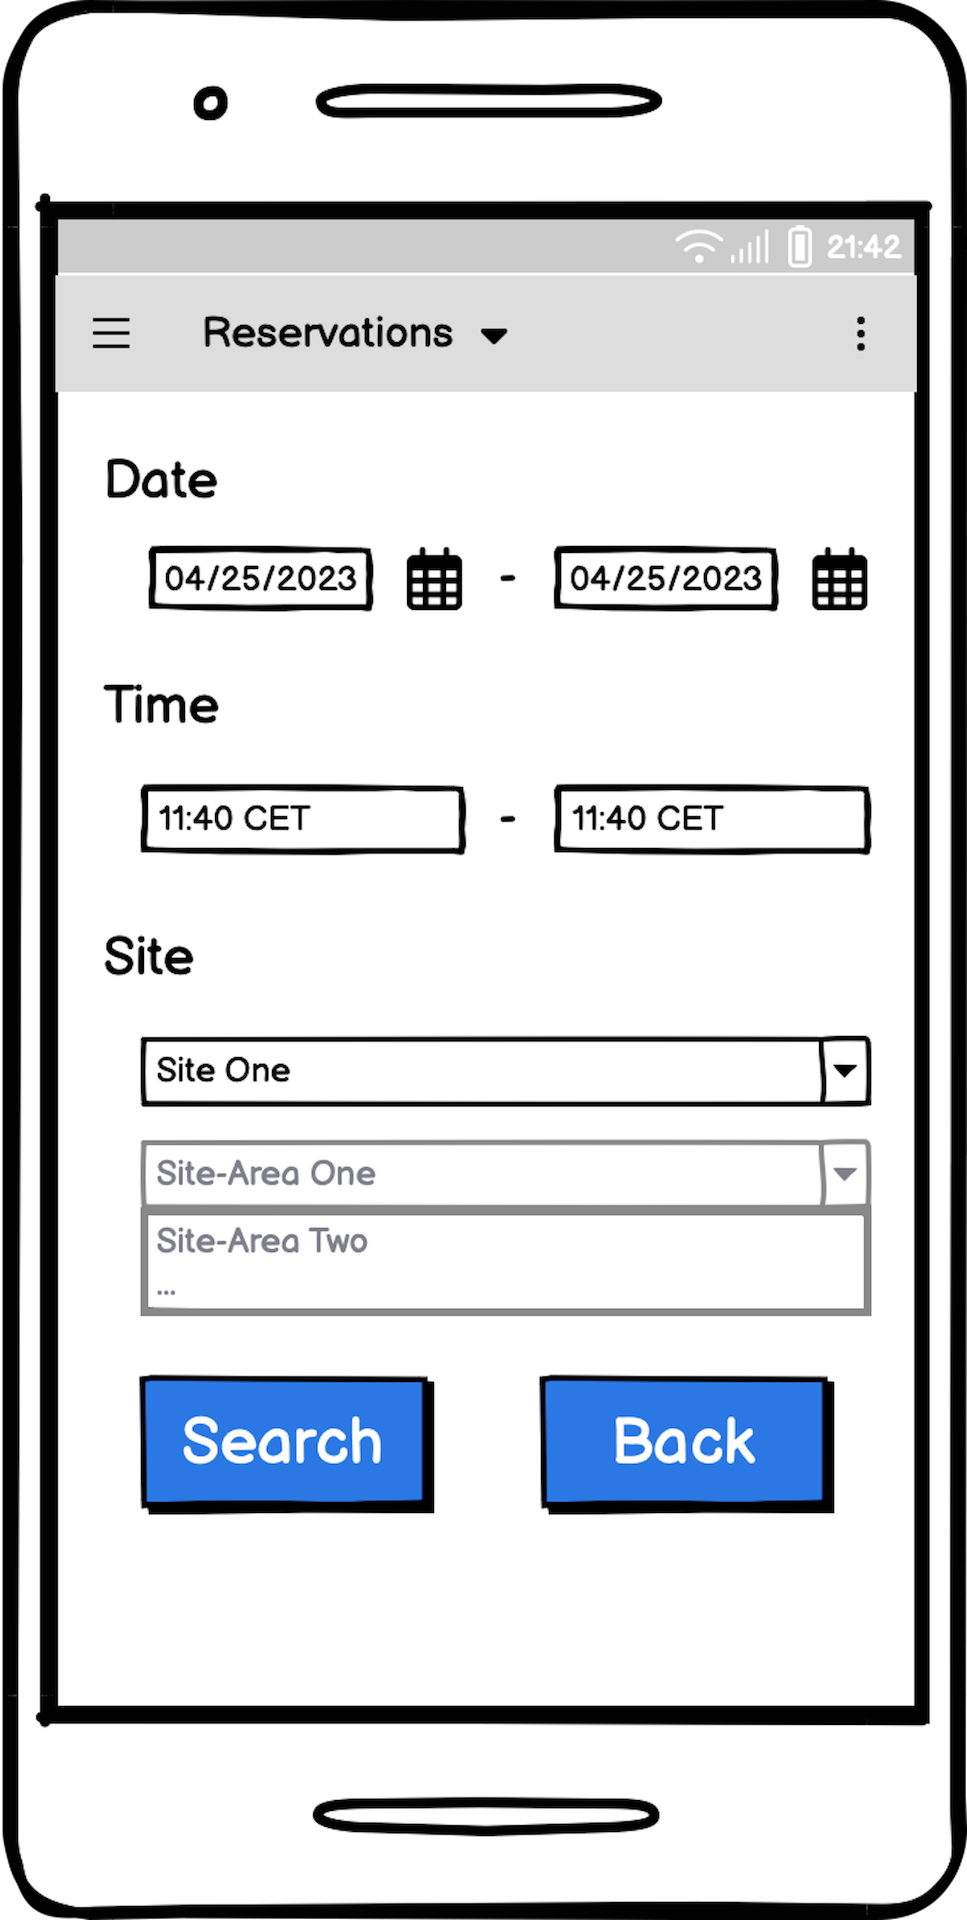
\includegraphics[width=\textwidth,height=1.6\textwidth,keepaspectratio]{resources/images/main/5_design/mockups/create_reservation/mobile/Create_Reservation.png}
        \caption{Create a reservation in the mobile application.}
        \label{fig:mobile-create-reservation}
    \end{subfigure}
    \caption{Mockups for the user interface of the mobile and web application relating to the creation of reservations.}
    \label{fig:mockups-create-reservation}
\end{figure}

\newpage

\subsubsection{Update Reservation}
\label{ch:Design:sec:Reservation System:ssec:Management Capabilities:sssec:Update Reservation}

To modify and manage existing reservations, the user is able to update a reservation. In addition to changing the date, time and \acrshort{cs}, modifications can be made to the connectors as well as the provided vehicle, if available. 
Similar to the creation process, the corresponding user input and changes are validated, resulting in further processing of the update process or immediate termination.
Referring to successful validation, the system searches for a reservation with the same \acrshort{id} to update it accordingly.
To capture potential events, such as unsaved reservations, the update process turns into the create process as described above to mitigate the erroneous behavior.
Otherwise, the reservation properties received are updated. If another time or \acrshort{cs} is selected, the reservation on the previous station is cancelled, and the newly selected \acrshort{cs} and connector are reserved.
Afterward, a series of steps similar to the creation process described above takes place. This includes checking for new collisions created by other users during the update and rejecting them accordingly, preparing the notifications for the selected \acrshort{cs}, and finally saving the updated reservation.
This also contains another notification that the user will receive upon successful completion.

\begin{figure}[h]
    \centering
    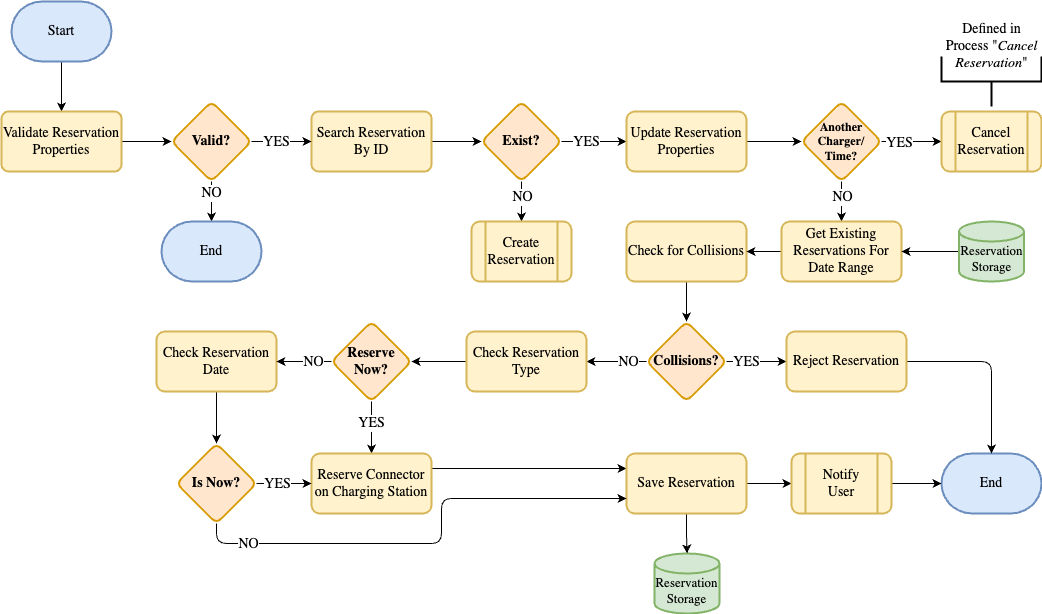
\includegraphics[scale=0.4]{resources/images/main/5_design/processes/ReservationUpdate.png}
    \caption{Process flow with all relevant steps to update a reservation.}
    \label{fig:update-reservation-flowchart}
\end{figure}

\noindent Due to a comparable range of input, the recommendations for the respective interfaces of the mobile and web applications are almost identical, as shown in Figure \ref{fig:mockups-update-reservation} below.

\begin{figure}[h]
    \centering
    \begin{subfigure}[c]{0.6\textwidth}
        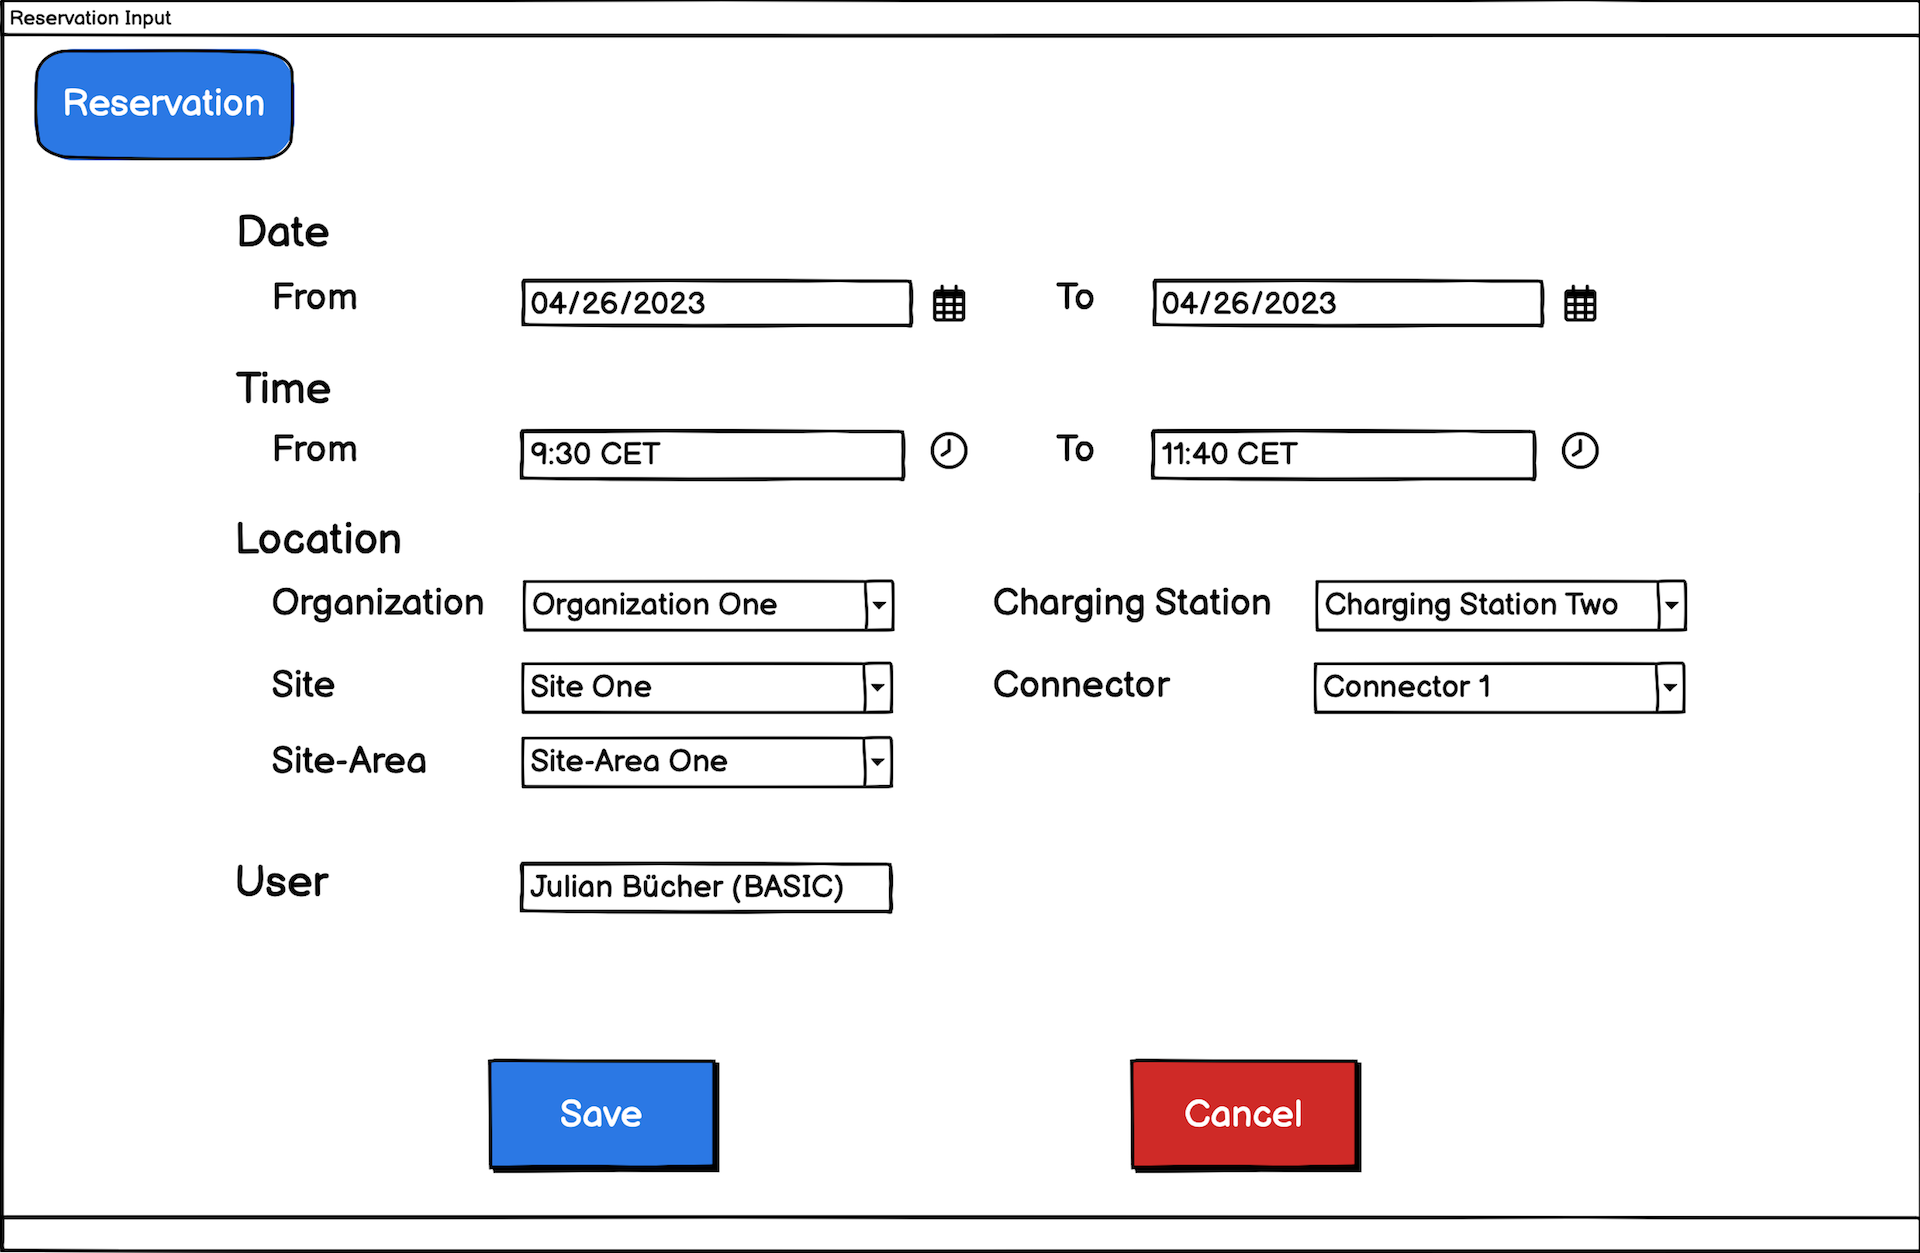
\includegraphics[width=\textwidth]{resources/images/main/5_design/mockups/update_reservation/web/Edit_Reservation.png}
        \captionsetup{skip=33pt}
        \caption{Update a reservation in the web application.}
        \label{fig:web-update-reservation-mockup}
    \end{subfigure}
     \hfill
     \begin{subfigure}[c]{0.3\textwidth}
         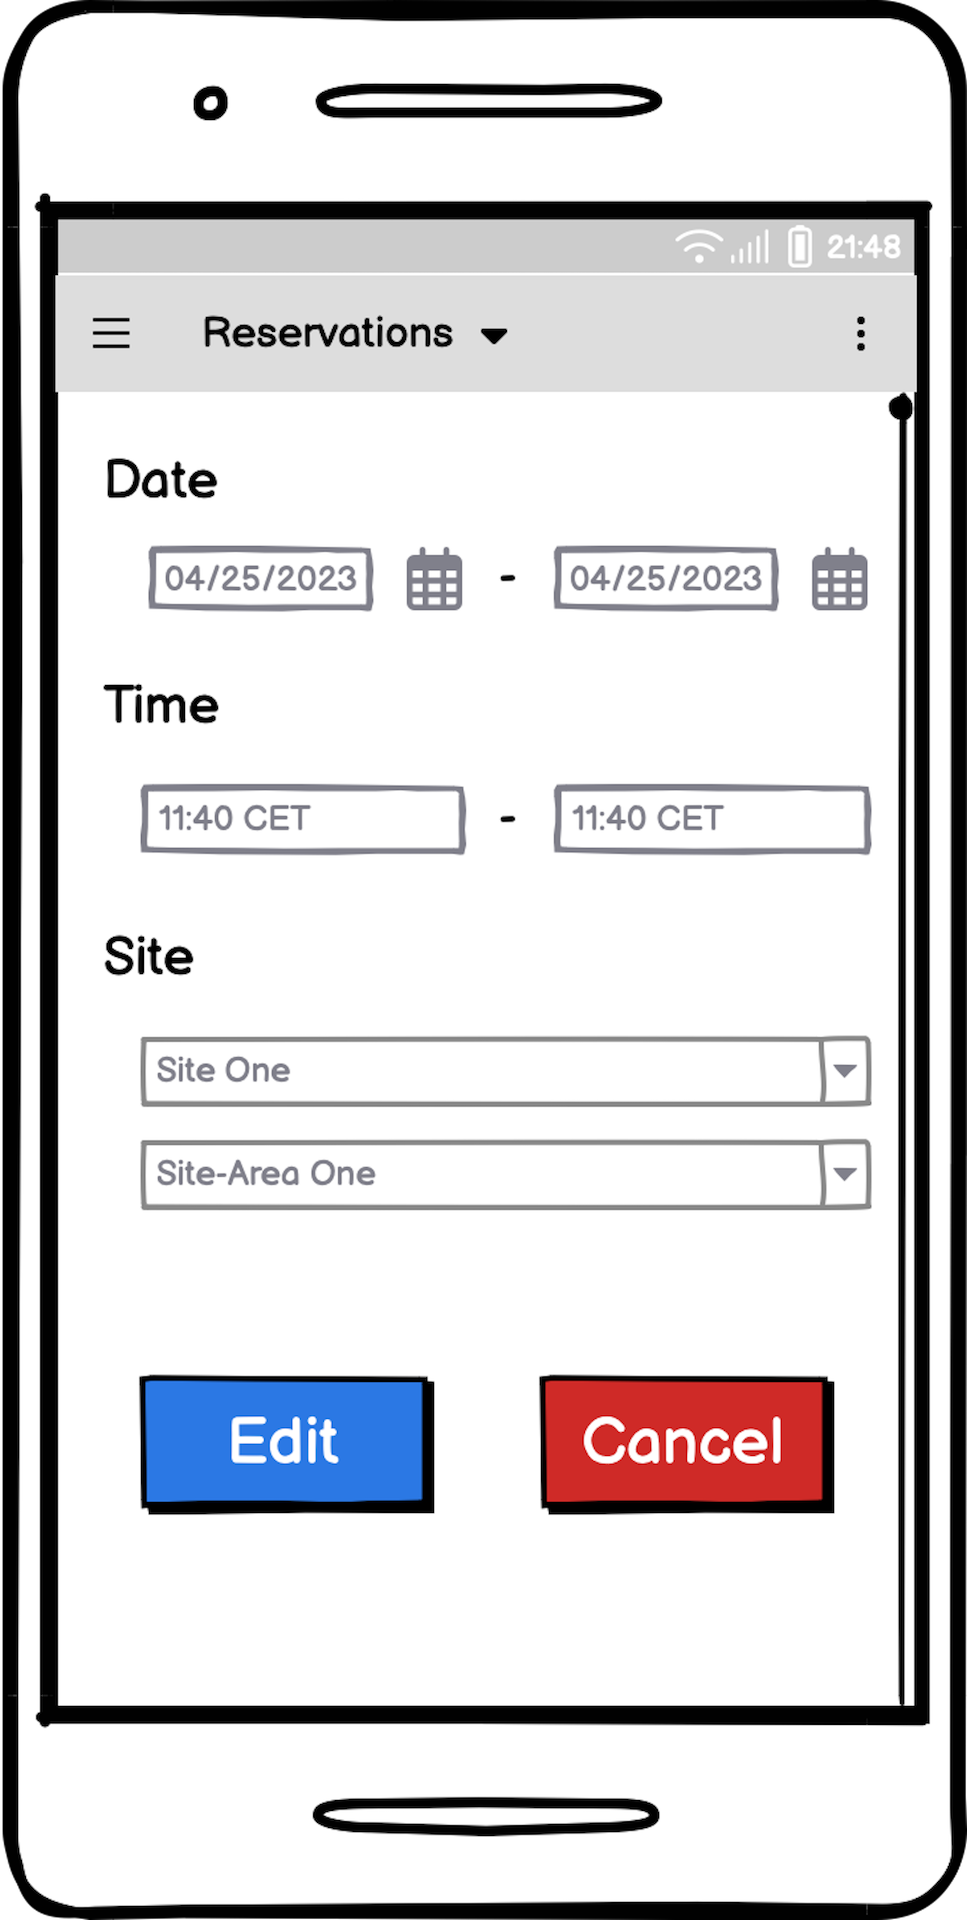
\includegraphics[width=\textwidth,height=1.6\textwidth,keepaspectratio]{resources/images/main/5_design/mockups/update_reservation/mobile/Edit_Reservation.png}
         \caption{Update a reservation in the mobile application.}
         \label{fig:mobile-update-reservation-mockup}
    \end{subfigure}
    \caption{Mockups for the user interface of the mobile and web application concerning the update of reservations.}
    \label{fig:mockups-update-reservation}
\end{figure}

\clearpage

\subsubsection{Cancel Reservation}
\label{ch:Design:sec:Reservation System:ssec:Management Capabilities:sssec:Cancel Reservation}

In addition to making a reservation, the user needs the option to cancel it in the case of changes due to unforeseen or unexpected circumstances.
To accomplish this task, the cancellation operation encapsulates the predefined \textit{Cancel Reservation} feature in \acrshort{ocpp} version 1.6 \cite{noauthor_ocpp_nodate}. As well as cancelling the active reservation on the \acrshort{cs}, it also allows cancelling scheduled reservations, taking into account the reservation life cycle as described in subsection \ref{ch:Design:sec:Reservation:ssec:Reservation Status}.
Initially, the designed process checks for an existing reservation with the same identifier in the database. If the reservation does not exist, the execution ends. This practice avoids the processing of unnecessary information and prevents communication with the corresponding customer service.
If the reservation exists, the reservation status is validated to cancel only reservations according to the predefined state transitions in Figure \ref{fig:reservation-states}. Furthermore, the current status of the reservation is determined, which results in a \textit{Cancel Reservation} request contacting the appropriate \acrshort{cs} if the reservation is in progress.
After the reservation status is set to \textit{Cancelled}, the reservation is saved once more, and a user notification containing the reservation's status transition is sent to the user.

\begin{figure}[h]
    \centering
    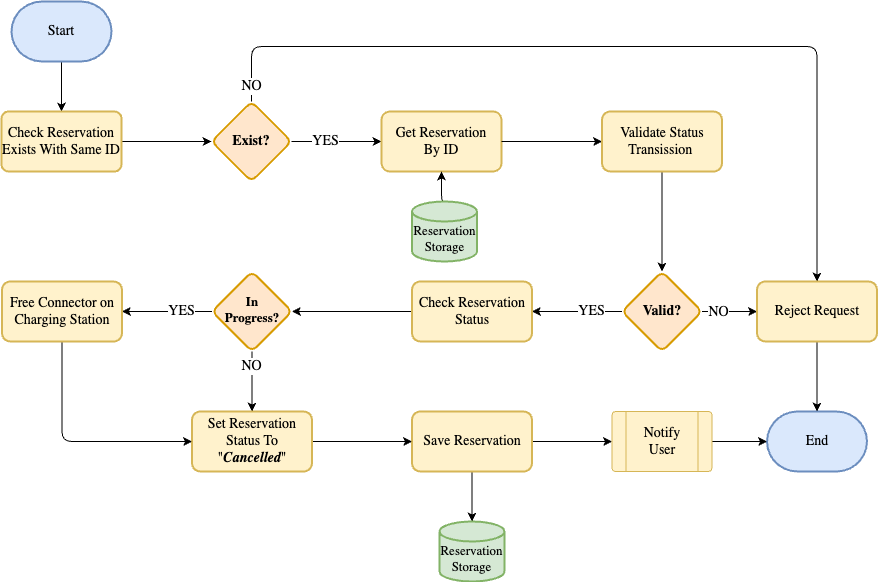
\includegraphics[scale=0.4]{resources/images/main/5_design/processes/ReservationCancel.png}
    \caption{Process flow with all according steps to cancel a reservation.}
    \label{fig:cancel-reservation-flowchart}
\end{figure}

\noindent By virtue of the atomic nature of this function, it is designed as a dedicated button within the mockups presented below. To confirm the cancellation of a reservation and complete the process, users will be presented with a confirmation dialogue in both applications, which is not displayed in the illustrations below.

\begin{figure}[h]
    \centering
     \begin{subfigure}[c]{0.6\textwidth}
         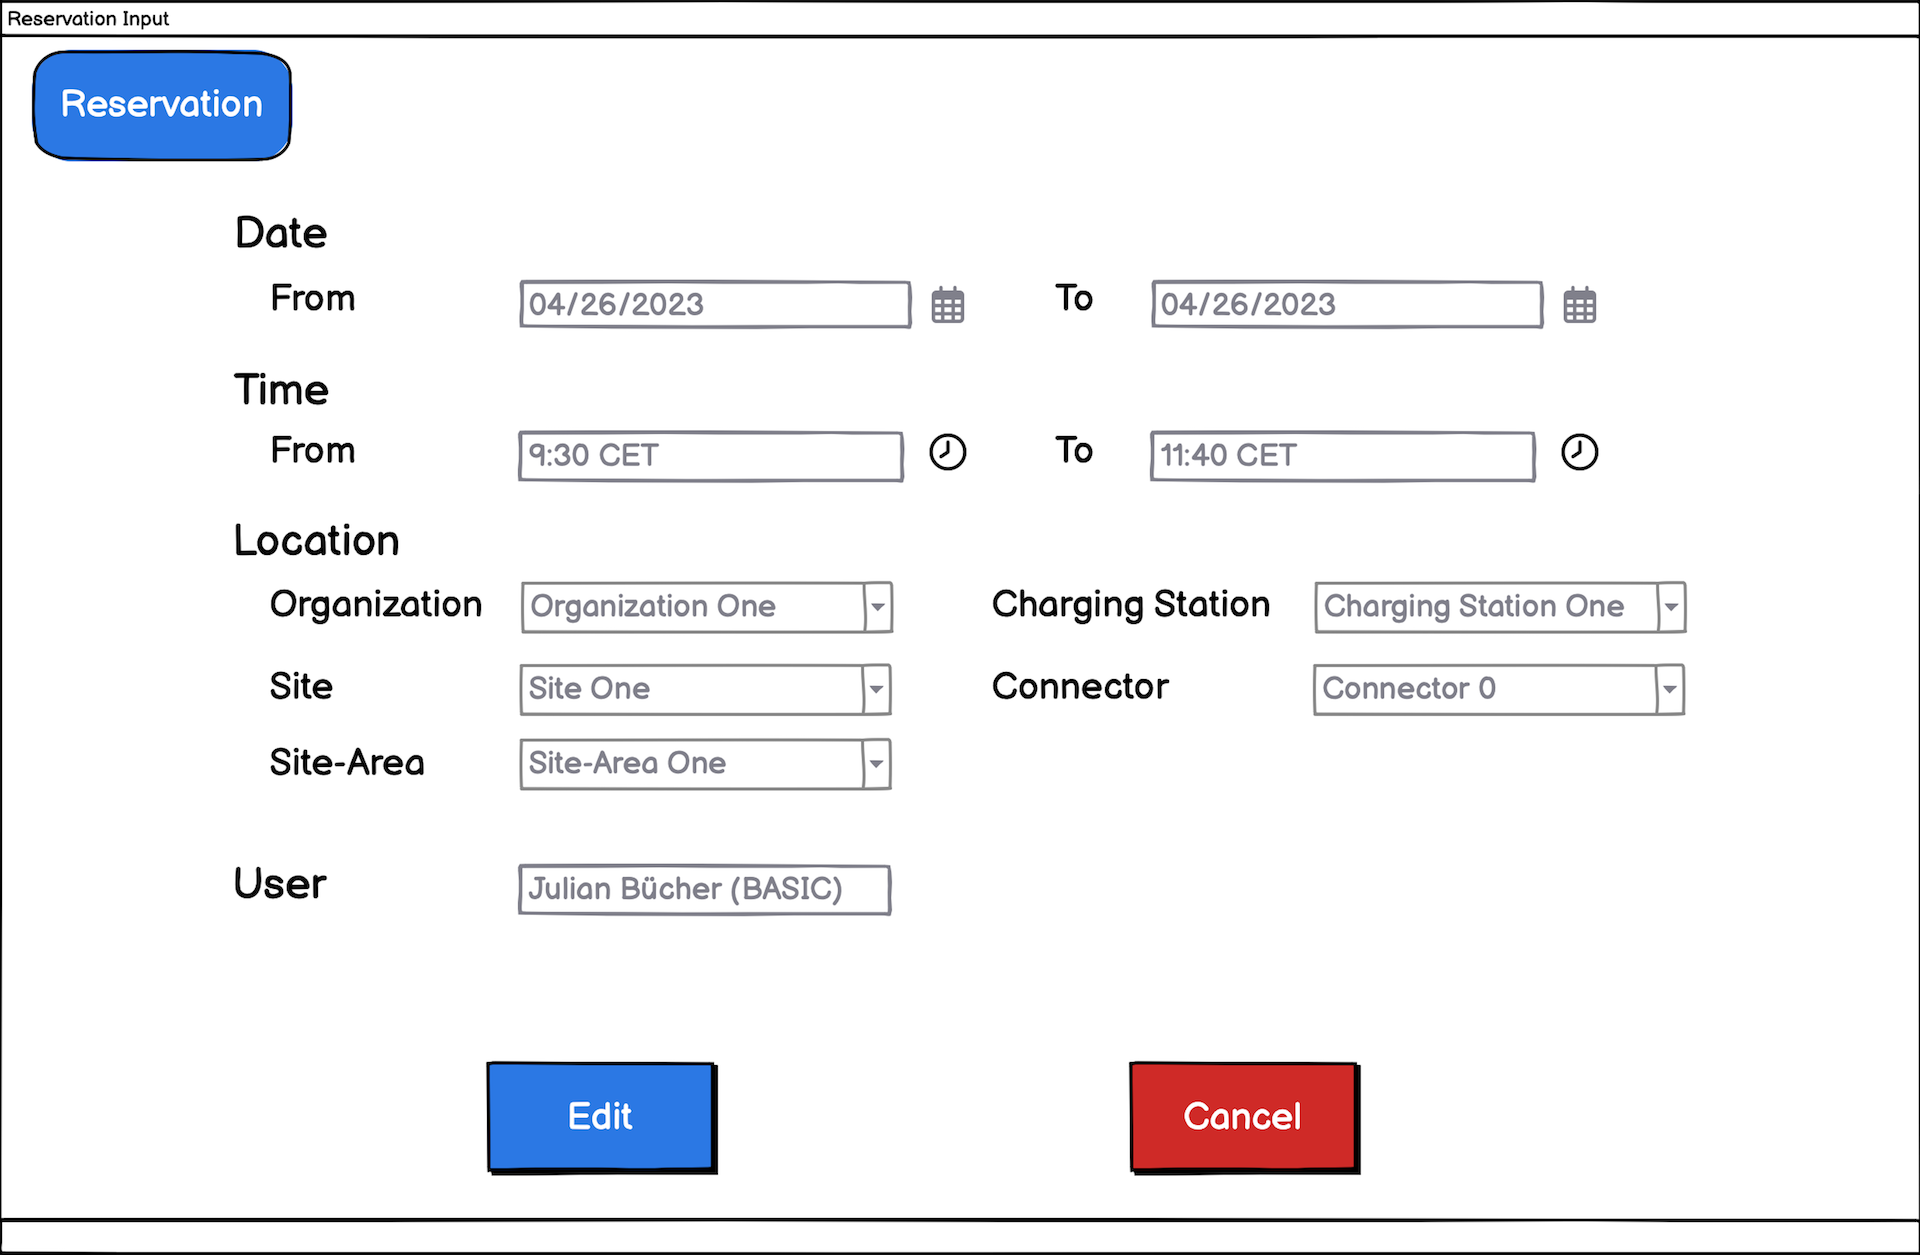
\includegraphics[width=\textwidth]{resources/images/main/5_design/mockups/cancel_reservation/web/Cancel_Reservation.png}
         \captionsetup{skip=33pt}
         \caption{Cancel a reservation in the web application.}
         \label{fig:web-cancel-reservation-mockup}
    \end{subfigure}
     \hfill
     \begin{subfigure}[c]{0.3\textwidth}
         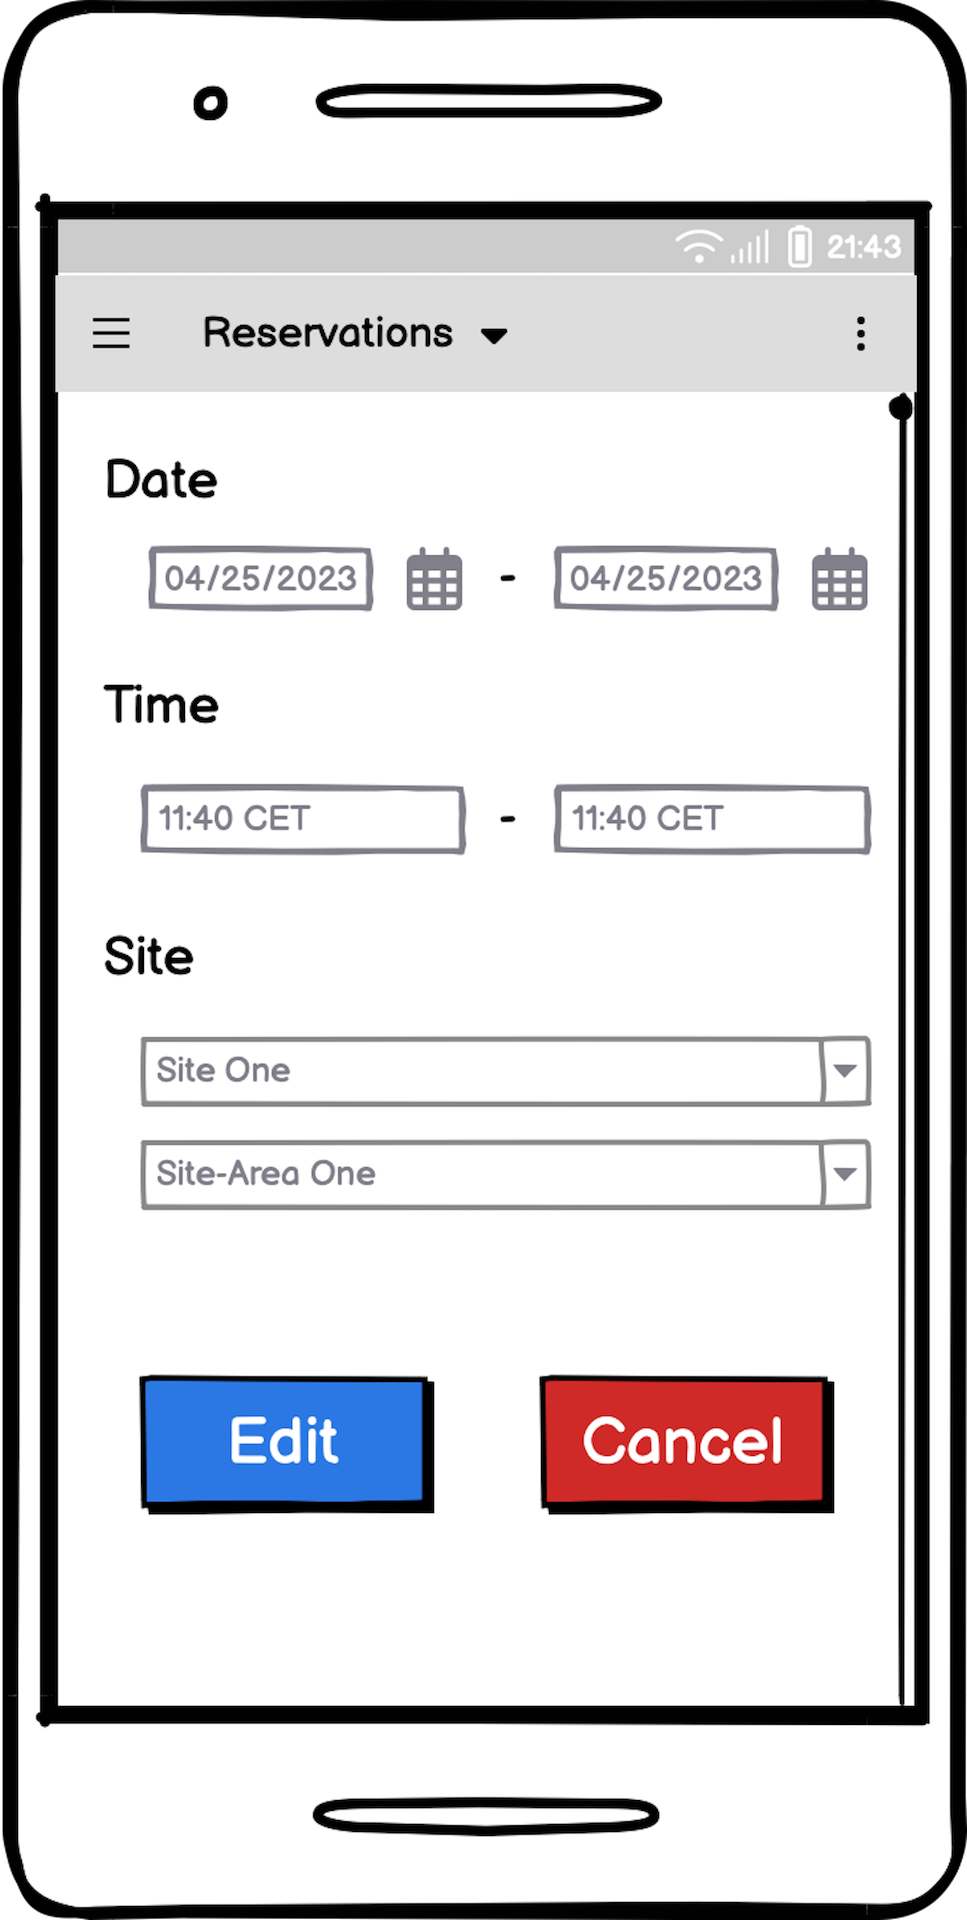
\includegraphics[width=\textwidth,height=1.6\textwidth,keepaspectratio]{resources/images/main/5_design/mockups/cancel_reservation/mobile/Cancel_Reservation.png}
         \caption{Cancel a reservation in the mobile application.}
         \label{fig:mobile-cancel-reservation-mockup}
    \end{subfigure}
    \caption{Mockups for the user interface of the mobile and web application in order to cancel a reservation.}
    \label{fig:mockups-cancel-reservation}
\end{figure}

\newpage

\subsubsection{Delete Reservation}
\label{ch:Design:sec:Reservation System:ssec:Management Capabilities:sssec:Delete Reservation}

Keeping in mind the management capabilities and complying with Article 17 of the \acrfull{gdpr}, which outlines the 'Right to Erasure' \cite{noauthor_art_2018}, the system offers the functionality to delete a reservation.
Aiming for comparable outcomes, this process operates in a similar fashion to the cancellation process explained previously, which also affects the design of the corresponding mockups.
Initially, the system storage is checked for the existence of the reservation identifier, which results in process termination if the reservation is not found. 
Otherwise, the reservation is queried and the reservation status is checked. If the status of the reservation is \textit{In Progress}, it is immediately cancelled. Afterward, the operation permanently deletes the record in the database. 

\begin{figure}[h]
    \centering
    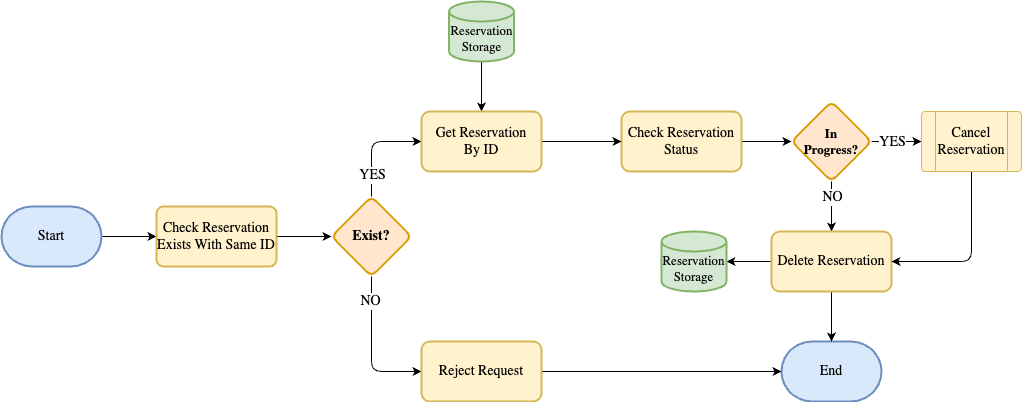
\includegraphics[scale=0.4]{resources/images/main/5_design/processes/ReservationDelete.png}
    \caption{Process flow with all according steps to delete a reservation.}
    \label{fig:delete-reservation-flowchart}
\end{figure}

\noindent As mentioned previously, no proposals have been made for the corresponding user interfaces. The author suggests that the delete feature could be implemented in a similar way to the \textit{Cancel Reservation} method discussed earlier, and does not require an additional design approach for the application interfaces.

\newpage

\subsubsection{Enable Reservations}
\label{ch:Design:sec:Reservation System:ssec:Management Capabilities:sssec:Enable Reservations}

Considering the reservation system as an independent part of the whole system, the user should have the possibility to activate or deactivate the respective functionality according to his needs.
To incorporate this functionality, it is presented as a toggle to control the operation of the reservation system with all its procedures. Similar to the approach presented in \cite{orcioni_ev_2020}, which describes the reservation system as a dedicated service. According to this proposal, it is possible to deactivate it as a module integrated as a subsystem.
This allows such functionality to be implemented alongside the processes described in existing standards, such as \acrshort{ocpp} or \acrshort{ocpi}, and does not interfere with their implementations.
Like the \textit{Delete Reservation} function, no user interface mockups are provided due to the simple nature of the function. In the subsequent implementation, this toggle should be considered within a central management interface that configures the functionalities of the different tenants. 

\newpage

\subsection{Scheduling Capabilities}
\label{ch:Design:sec:Reservation System:ssec:Scheduling Capabilities}

To address the scheduling capabilities discussed in subsection \ref{ch:Design:sec:Reservation System:ssec:Design Criteria}, the subsequent procedures have been developed to manage reservations independently.
This should enable the system to maintain a consistent state and autonomously manage the associated charging infrastructure.
For this purpose, the scheduling, expiry, and release procedures are created to handle the reservations according to their current state.

\subsubsection{Schedule Reservation}
\label{ch:Design:sec:Reservation System:ssec:Scheduling Capabilities:sssec:Schedule Reservation}

By utilizing the scheduling process, the system identifies present and forthcoming reservations from the database according to a pre-defined threshold. 
If there are no upcoming reservations in the near future, the scheduler process is terminated, otherwise, the \acrshortpl{cs} and connectors defined in each reservation are reserved.
Similar to the create and update functions described within the management capabilities subsection \ref{ch:Design:sec:Reservation System:ssec:Management Capabilities}, the \acrshort{ocpp} \textit{ReserveNow} operation \cite{noauthor_ocpp_nodate} is implemented to provide standards-compliant communication between the reservation system and the \acrshort{cs}.
If connectors are in an occupied state, the \textit{Stop Transaction} operation is performed, resulting in an immediate termination of the current charging session and returning the \acrshort{cs} to an available state.
Allowing the system to carry out the upcoming reservation on the released connector, resulting in the \acrshort{cs} accepting the \textit{ReserveNow} request.
Consequently, the reservation status is updated to \textit{In Progress} and saved once again.

\begin{figure}[h]
    \centering
    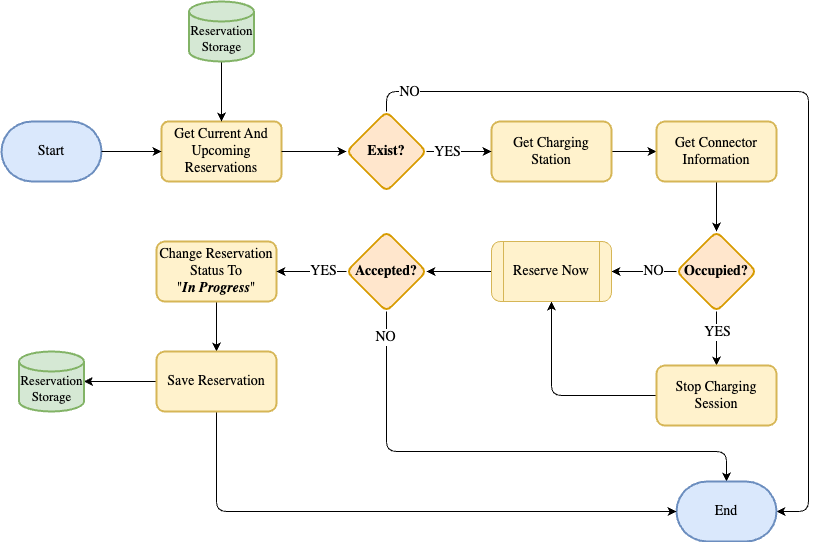
\includegraphics[scale=0.4]{resources/images/main/5_design/processes/scheduler/SynchronizeReservation.png}
    \caption{Process for scheduling upcoming reservation on a specified \acrshortpl{cs}.}
    \label{fig:schedule-reservation-flowchart}
\end{figure}

\noindent Besides providing autonomous functionality for synchronizing reservations with the corresponding \acrshortpl{cs}, this procedure allows the execution of recurring reservations during the defined period. 
Furthermore, if the user disconnects the connector during the reservation period, the underlying logic ensures that the reservation remains active until a certain threshold is reached.

\subsubsection{Expire Reservation}
\label{ch:Design:sec:Reservation System:ssec:Scheduling Capabilities:sssec:Expire Reservation}

Forming the counterpart to the scheduling process, which synchronises upcoming and ongoing reservations with the \acrshortpl{cs}, the expiring process handles all reservations that are neither cancelled nor expired and have reached their expiration date.
The process ends immediately upon discovering any such reservations. Otherwise, the status of the reservation is changed to \textit{Expired}, the user is notified and the reservation is saved again.

\begin{figure}[h]
    \centering
    
\includegraphics[scale=0.4]{resources/images/main/5_design/processes/scheduler/UpdateExpiredReservations.png}
    \caption{Process flow for reservations reaching their expiration date.}
    \label{fig:expire-reservation-flowchart}
\end{figure}

\noindent In cooperation with the \textit{Free Reserved Connector} procedure described in the sub-subsection \ref{ch:Design:sec:Reservation System:ssec:Scheduling Capabilities:sssec:Free Reserved Connector}, the \textit{Expire Reservation} procedure handles the transition from the active state to a final state that invalidates the reservation.
Using the \textit{Expired} status handles reservations that are not correctly updated according to the \textit{Done}, \textit{Cancelled} or \textit{Unmet} states, caused by information or connection loss between the management instance and the \acrshort{cs}.
This approach ensures that concurrent active reservations are minimized and provides a sort of self-healing process to clean up the growing data store.

\subsubsection{Free Reserved Connector}
\label{ch:Design:sec:Reservation System:ssec:Scheduling Capabilities:sssec:Free Reserved Connector}

In the case of a reserved connector being blocked, the respective user who made the booking did not show up and failed to cancel the reservation, thus preventing the connector from being available again.
To reduce the likelihood of this situation, the system provides a process to automatically remove unmet reservations from the \acrshortpl{cs} and associated connectors.
In order to identify these bookings, the system selects reservations that are already in progress, the connector is not in the \textit{Charging} state and the specified arrival time is overdue by a certain threshold.
After identifying reservations that meet these criteria, the system cancels them on the \acrshortpl{cs}. Once the station successfully acknowledges the cancellation, the reservation status is updated to \textit{Unmet}.
Otherwise, the process ends immediately. The same rule applies if the \acrshort{cs} does not permit the cancellation of the reservation.

\begin{figure}[h]
    \centering
    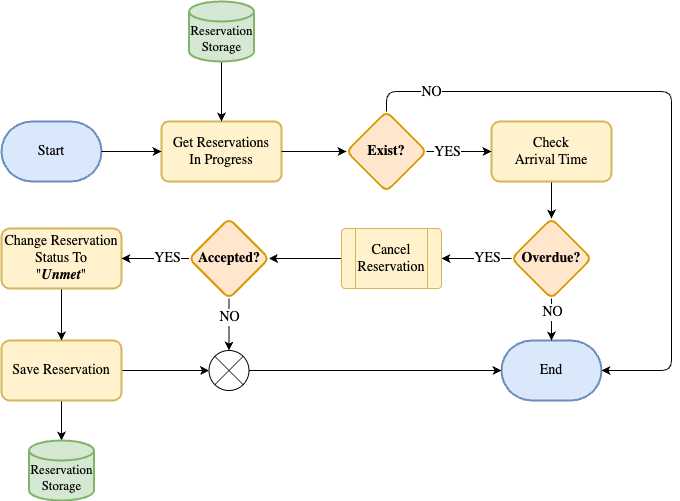
\includegraphics[scale=0.4]{resources/images/main/5_design/processes/scheduler/CancelUnmetReservation.png}
    \caption{Process flow for releasing connectors with unfulfilled reservations.}
    \label{fig:free-connector-flowchart}
\end{figure}

\newpage

\subsection{Notification Capabilities}
\label{ch:Design:sec:Reservation System:ssec:Notification Capabilities}

Besides the management and automation techniques presented above, the exchange of information with the user encompasses one aspect of the predetermined design parameters.
Concerning the methods in \cite{zarkeshev_charging_2018}, the reservation system should interact with the user in a certain way to inform him or her about upcoming reservations or schedule changes, which the user should consider for further planning activities.
For this reason, this system design outlines several scenarios that are considered by the author to be relevant for the reservation system to inform the user according to the changes made to the reservations. 
This also satisfies the aspects of the \textit{Data Availability} design parameter in a more general sense. Within the scope of the aforementioned work, this parameter is limited solely to data regarding the status of charging stations and connectors. However, additional expansions could be made to include data on reservation statuses.
For a clearer insight into the constraints associated with each notification type, a brief explanation of the concerning scenarios is succeeding. 

\subsubsection{Reservation Status Changed}
\label{ch:Design:sec:Reservation System:ssec:Notification Capabilities:sssec:Reservation Status Changed}

Besides the users' ability to manually configure their reservations, the bulk of the work is performed by background tasks that run in parallel to the main processes.
For standard users, it is neither feasible nor beneficial to regularly monitor the status of their reservations on their own. Thus, it is necessary to send notifications containing information about changes in the status of a reservation throughout its life cycle.
Due to its supportive role within the system context, this type of functionality could be integrated into one of the previously designed processes. 
Considering an intended integration, the next parts of the design processes could be proposed as suitable extension points using the notification capabilities within \textit{Schedule Reservation}, \textit{Expire Reservation}, and \textit{Free Reserved Connector}.

\subsubsection{Reservation Upcoming}
\label{ch:Design:sec:Reservation System:ssec:Notification Capabilities:sssec:Reservation Upcoming}

To address the emergence of reservations, two distinct types of notifications can be extracted from the more generic one. One is the notification of the user to whom the reservation belongs and the other is the notification of the user who intends to charge at a \acrshort{cs} if a reservation comes up in the near future. 
Both scenarios are represented by the notification type of a \textit{Reservation Upcoming}.

\begin{description}
    \item[Upcoming Reservation Notification] According to the process of scheduling reservations, users must receive a notification if their reservation is due to start in the near future. This type of notification should provide the user with the relevant metadata about the reservation and its commencement, ensuring they are informed about the upcoming reservation.
    \item[Upcoming Reservation Warning] Message that the charging station that the driver is currently using has a reservation in the pipeline that conflicts with the estimated duration of the charging session. This should persuade the driver to consider relocating his car. Otherwise, the charging session is stopped when the reservation starts, and the \acrshort{ev} is no longer charged, making it pointless to occupy this station.
\end{description}

\noindent Locating these specific notification types, using them within the \textit{Schedule Reservation} feature as part of the previously mentioned designs might be the best option.

\subsubsection{Charging Station Blocked}
\label{ch:Design:sec:Reservation System:ssec:Notification Capabilities:sssec:Charging Station Blocked}

Considering the \textit{Upcoming Reservation Warning} mentioned previously, only the user occupying the reserved \acrshort{cs} is notified that it is potentially blocking a reserved port. To complement this scenario, the user of the upcoming reservation belongs to requires a notification as well.
To guarantee that the user is informed of the occurrence of unintended behavior, the \textit{Charging Station Blocked} notification fulfills the objective of the desired information flow. In this way, if the \acrshort{cs} is still blocked and the other \acrshort{evu} does not remove the car from the parking lot accordingly, the notified user is able to switch the reservation to another available \acrshort{cs} in that area.
Despite stopping the charging session in accordance with the \textit{Schedule Reservation} process, the car could still end up blocking the car bay for the arriving user, resulting in a negative user experience. Therefore, the system is intended to provide such mitigation techniques to inform the user in advance and allow him or her to adjust the reservation.
Considering the integration of this particular notification, the \textit{Schedule Reservation} as a part of the designed processes seems appropriate.

\subsubsection{Reservation Cancelled}
\label{ch:Design:sec:Reservation System:ssec:Notification Capabilities:sssec:Reservation Cancelled}

When considering the \textit{Reservation Status Changed} notification introduced earlier, this notification type seems to be a duplicate of a still--existing function.
However, there should be a specific notification in the system design to inform the user when a reservation is being cancelled. The system's implementation and internal administrative structure do not allow only the user who created the reservation to cancel it. 
If an administrator performs this operation, the user should also be notified that their reservation is about to be cancelled. 
That is why this notification introduces an extension to the changing status notification, in order to deliver this information.
Based on the intended use, the \textit{Cancel Reservation} function permits an appropriate integration of this notification.

\subsubsection{Reservation Unmet}
\label{ch:Design:sec:Reservation System:ssec:Notification Capabilities:sssec:Reservation Unmet}

Based on the same idea as the \textit{Reservation Cancelled} message, this kind of notification enables the system to inform the user about unwanted behavior.
When a user fails to arrive within the designated time frame for their reservation, the \textit{Free Reserved Connector} process usually takes care of these reservations. 
However, given the damaging effects of such a behaviour, like blocking a charging session that could be used by another user, and the associated loss of profit, when combined with the charges for the reservation.
To reduce the occurrence of such actions, the system should send a message advising the user that their current reservation is no longer viable according to this process. Furthermore, it should be accompanied by a warning to remind the user to cancel a reservation if he or she no longer demands it, to cultivate more altruistic behavior.
As previously mentioned, the \textit{Free Reserved Connector} enables the proper use of this notification type. \\ \\
\noindent The integration possibilities and application domains addressed in this chapter are derived from the current state of the standards used in this thesis and are based on the considerations and design principles available at this stage of the design work. 
As these functionalities and features are evolving, their use could be extended to other areas and related systems.
